%% TIPO DE DOCUMENTO 

\documentclass{beamer}

\usetheme{Madrid}
\usecolortheme{seagull}
\usefonttheme{professionalfonts}

%%% IMPORTAMOS PAQUETES A USAR 

\usepackage[utf8]{inputenc}
%\usepackage[latin1]{inputenc}
\usepackage[spanish, es-tabla]{babel}
\usepackage{csquotes}
\usepackage{float}
\usepackage{graphicx}
\usepackage{hyperref}
%Pruebas para animaciones
\usepackage{animate}
\usepackage[document]{ragged2e}
\usepackage{bibentry}
\usepackage{graphicx} % Allows including images
\usepackage{booktabs} % Allows the use of \toprule, 

%%%START APA
%\usepackage[british]{babel}
%\usepackage[backend=biber,style=apa]{biblatex} OJO CON ESTA LINEA
\setbeamertemplate{navigation symbols}{} % To remove the navigation symbols from the bottom of all slides uncomment this line
%\DeclareLanguageMapping{british}{british-apa}
%\addbibresource{references.bib}
%% APA citing
%% \cite{t} - Uthor und Richter, 2010
%% \textcite{t} - Uthor und Riter (2010)
%% \parencite{t} - (Uthor & Riter, 2010)
%% \parencite[Chapt.~4]{t} - (Uthor & Riter, 2010, S. 15)
%%%END APA

%%%%% =================  PORTADA ================== 

\title[Sesión 2] 
{Movimientos de la Tierra}
%\subtitle {ne compléter que si l'article possède un sous-titre}

\author[Victor M. Santos] 
%\author[Pedro A. Salgado-Meza ]
{Victor M. Santos \inst{} \and M.Tarazona-Alvarado \inst{} \and J. Pisco-Guabave \inst{}} %\inst{1} \inst{3}}
%{P. A. ~Salgado-Meza\inst{1} \inst{2}}%\and I.~Borne\inst{1} \and J.~Buisson\inst{2}}

\institute[]{
\inst{}Grupo Halley, Escuela de Física, Universidad Industrial de Santander, Bucaramanga, Colombia.}
%\institute[]
%{
%  \inst{1}%
%  Universidad Industrial de Santander, Bucaramanga, Colombia
%  \and
%  \inst{2}%
%  Escuela de Ingenierías Eléctrica, Electrónica y Telecomunicaciones
%  \and
%  \inst{3}%
%  Escuela de Ingeniería Mecánica  
%  }

\date{ }



\begin{document}
\logo{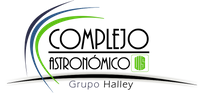
\includegraphics[scale=0.3]{Imagenes/Logo_Halley}} 


\begin{frame}
\titlepage % Print the title page as the first slide
\end{frame}

%%%%%%%%%%%%%%%%%%%%%%%%%%%%%%%%%%%%%%%%%%%%%%%%%%%%%%%%%%%%%%%%%%%%%%%%%%%%%%%%%%%%%%%%%%%%%%%%%%%%%%
\begin{frame}{Rotación}
 \begin{columns}
 \column{.45\textwidth}
  \begin{figure}
   \centering
   %\raggedright
   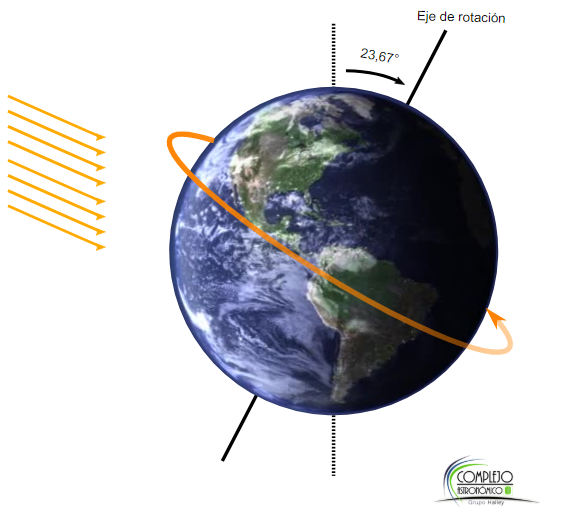
\includegraphics[scale=0.3]{Imagenes/Rotacion_01}
  \end{figure}
 \column{.45\textwidth}
 \small
 \justify
\begin{itemize}
\item La rotación de la Tierra es sobre su eje
\item Se define que el día dura aproximadamente 24 horas
\item Los astros en el firmamento se desplazan hacia el Oeste
\end{itemize}
 \end{columns}
\end{frame}

\begin{frame}
 \begin{columns}
 \column{.45\textwidth}
  \begin{figure}
   \centering
   %\raggedright
   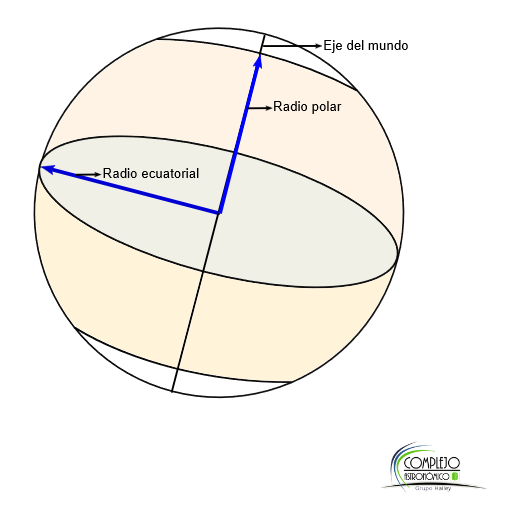
\includegraphics[scale=0.4]{Imagenes/Achatamiento_01}
  \end{figure}
 \column{.45\textwidth}
 \small
 \justify
\begin{itemize}
\item Achatamiento de la Tierra
\item La Tierra tiene forma de \textbf{geoide}
\end{itemize}
 \end{columns}
\end{frame}

\begin{frame}{Traslación}
 \begin{columns}
 \column{.45\textwidth}
  \begin{figure}
   \centering
   %\raggedright
   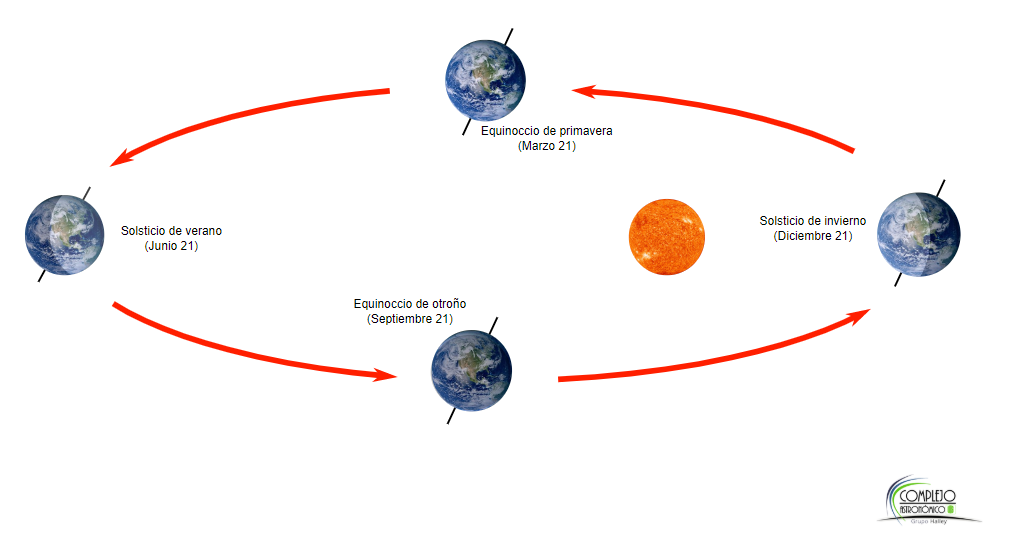
\includegraphics[scale=0.2]{Imagenes/Traslacion_01}
  \end{figure}
 \column{.45\textwidth}
 \small
 \justify
\begin{itemize}
\item La Tierra describe una órbita elíptica con el Sol en uno de sus focos
\item Se define que el año dura aproximadamente 365 días
\item Permite la existencia de las estaciones en la Tierra
\end{itemize}
 \end{columns}
\end{frame}

\begin{frame}
 \begin{columns}
 \column{.45\textwidth}
  \begin{figure}
   \centering
   %\raggedright
   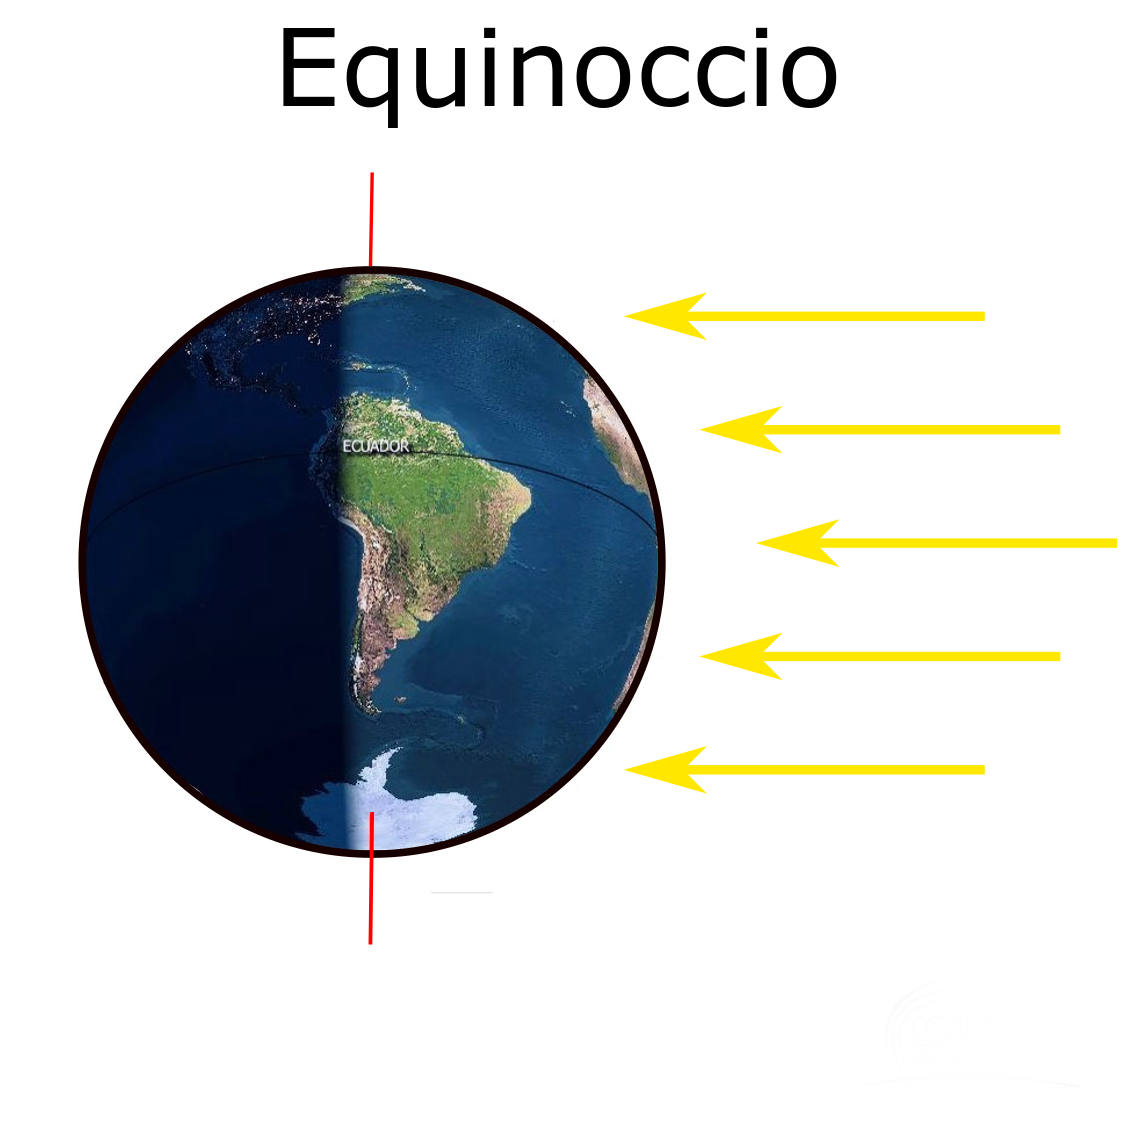
\includegraphics[scale=0.14]{Imagenes/Equinoccio}
  \end{figure}
 \column{.45\textwidth}
\begin{figure}
   \centering
   %\raggedright
   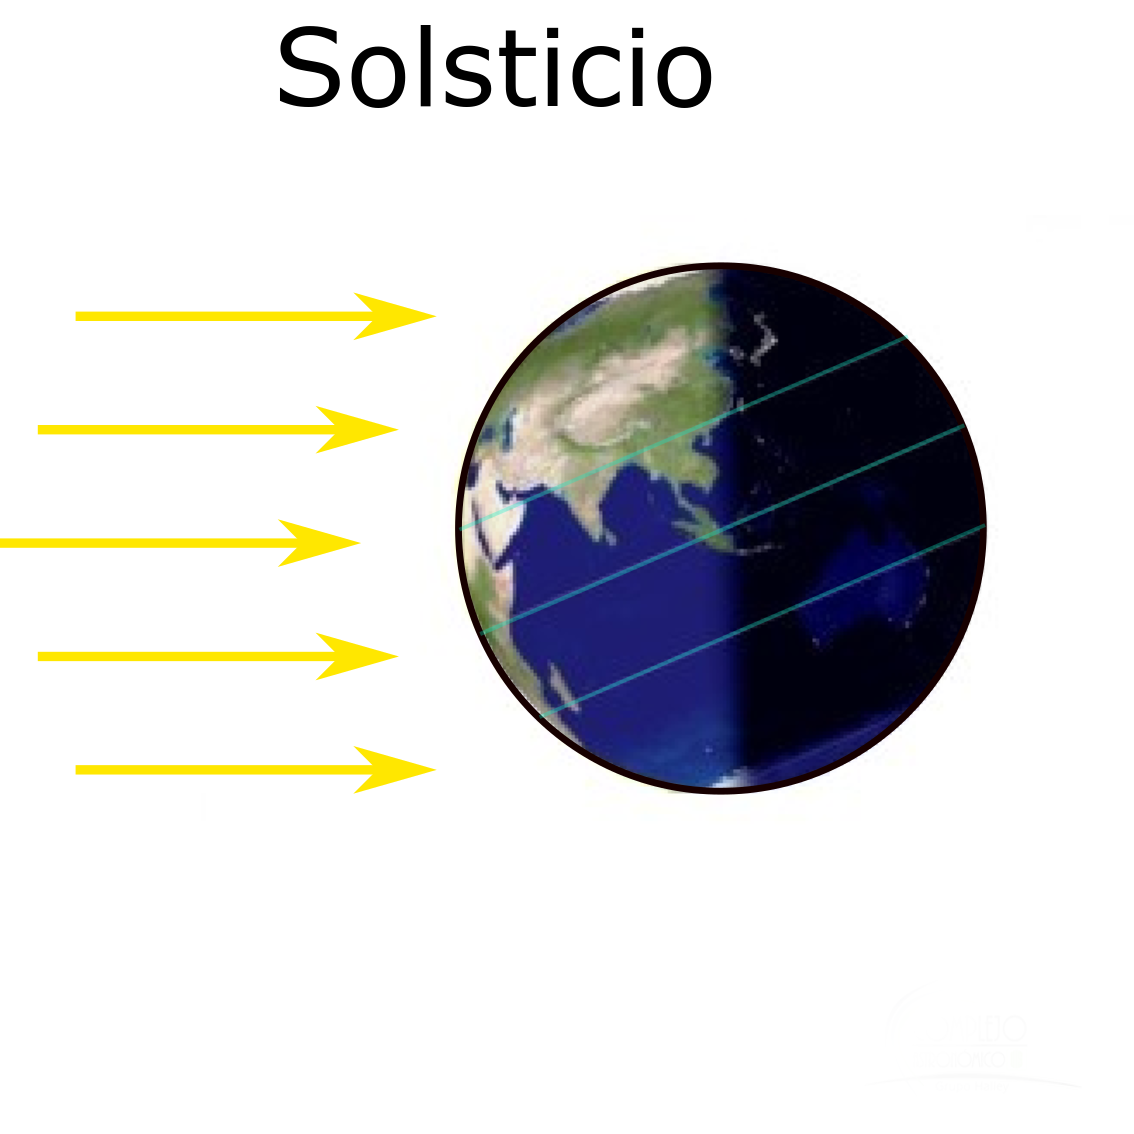
\includegraphics[scale=0.14]{Imagenes/solsticio}
  \end{figure}
 \end{columns}
\end{frame}


\begin{frame}{Precesión}
 \begin{columns}
 \column{.45\textwidth}
  \begin{figure}
   \centering
   %\raggedright
   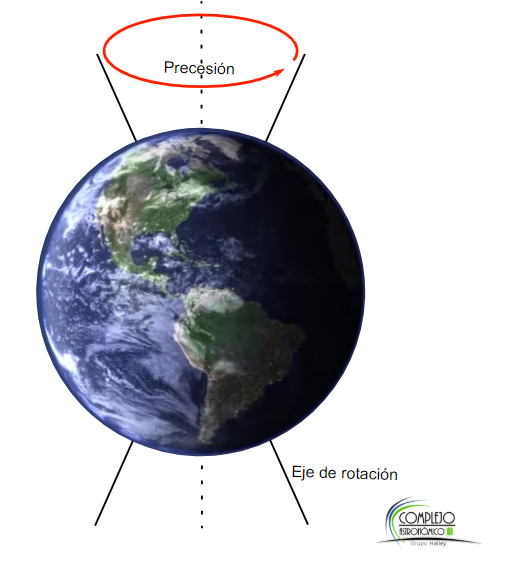
\includegraphics[scale=0.35]{Imagenes/Precesion_01}
  \end{figure}
 \column{.45\textwidth}
 \small
 \justify
\begin{itemize}
\item Cambio de dirección que experimenta el eje de rotación del planeta tierra
\item Se repite cada 25.800 años con dirección antihoraria
\end{itemize}
 \end{columns}
\end{frame}

\begin{frame}{Nutación}
 \begin{columns}
 \column{.45\textwidth}
  \begin{figure}
   \centering
   %\raggedright
   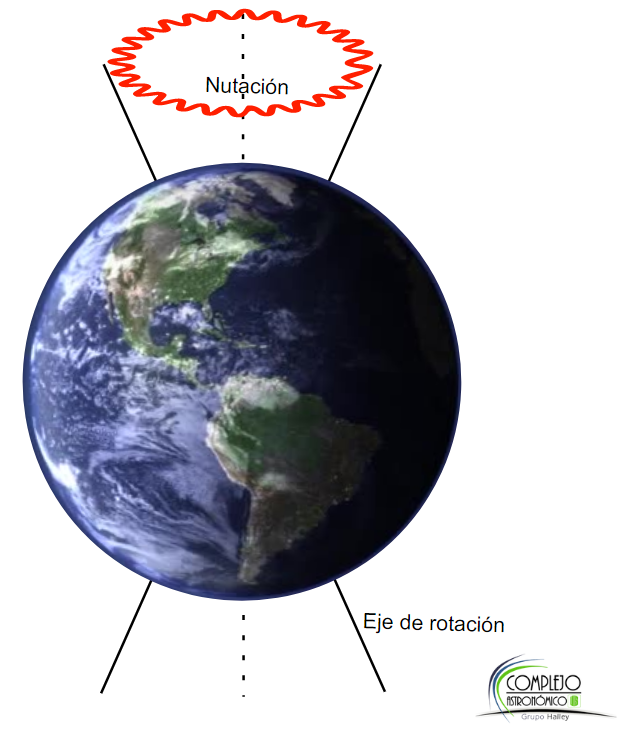
\includegraphics[scale=0.3]{Imagenes/Nutacion_01}
  \end{figure}
 \column{.45\textwidth}
 \small
 \justify
\begin{itemize}
\item Es causado directamente por la influencia gravitatoria de la Luna
\item La Tierra presenta oscilaciones que causan una mayor o menor inclinación del eje de la Tierra
\end{itemize}
 \end{columns}
\end{frame}

\begin{frame}
\begin{center}
\Huge 
\textit{``La naturaleza nunca hace nada superfluo, nada inútil, y sabe sacar múltiples efectos de una sola causa"}
\end{center}
\begin{flushright}
\small
\textit{Nicolás Copérnico}
\end{flushright}
\end{frame}

\end{document}